%%%%%%%%%%%%%%%%%%%%%%%%%%%%%%%%%%%%%%%%%
%
% (c) 2022 by Jennifer Laaser
%
% This work is licensed under the Creative Commons Attribution-NonCommercial-ShareAlike 4.0 International License. To view a copy of this license, visit http://creativecommons.org/licenses/by-nc-sa/4.0/ or send a letter to Creative Commons, PO Box 1866, Mountain View, CA 94042, USA.
%
% The current source for these materials is accessible on Github: https://github.com/jlaaser/pogil-polymers
%
%%%%%%%%%%%%%%%%%%%%%%%%%%%%%%%%%%%%%%%%%

\renewcommand{\figpath}{content/polymchem/livingpolyms/ringopening/figs}
\renewcommand{\labelbase}{ringopening}

\begin{activity}{Ring-Opening Polymerizations}

\begin{instructornotes}
	This activity introduces students to concepts related to ring-opening polymerizations.
	
	After completing this activity, students will be able to:
	\begin{enumerate}
		\item Explain the thermodynamic driving forces for ring-opening polymerizations, and predict a monomer's propensity to polymerize from its ring strain
		\item Predict the polymer produced by ring-opening metathesis polymerization of a given monomer, and predict the monomer needed to produce a target polymer
		\item Explain the mechanism of the metal-catalyzed polymerization of polylactide
	\end{enumerate}
	
	\subsection*{Activity summary:}
	\begin{itemize}
		\item \textbf{Activity type:} Learning Cycle
		\item \textbf{Content goals:} See above
		\item \textbf{Process goals:} %https://pogil.org/uploads/attachments/cj54b5yts006cklx4hh758htf-process-skills-official-pogil-list-2015-original.pdf
			\begin{itemize}
				\item Reading and interpreting reaction mechanisms
				\item Analyzing quantitative data
				\item Oral and written communication of reasoning
			\end{itemize}
		\item \textbf{Duration:} 60 minutes, including class discussion
		\item \textbf{Instructor preparation required:} none beyond knowledge of relevant content
		\item \textbf{Related textbook chapters:}
			\begin{itemize}
				\item \emph{Polymer Chemistry} (Hiemenz \& Lodge), 2nd ed.: section 4.8
				\item \emph{Introduction to Polymers} (Young \& Lovell), 3rd ed.: sections 7.1 and 7.5 %note: does not discuss thermodynamics in detail...
			\end{itemize}
		%\item \textbf{Facilitation notes:}
		%	\begin{itemize}
		%		\item \dots
		%	\end{itemize}
	\end{itemize}
	
\end{instructornotes}


\begin{model}[Fundamentals of Ring-Opening Polymerizations]
	\label{\labelbase:mdl:ROP}

	Ring-opening polymerizations are polymerizations in which a cyclic (ring-shaped) monomer is opened up to form a linear segment of the polymer backbone, as shown below:
	
	\centerline{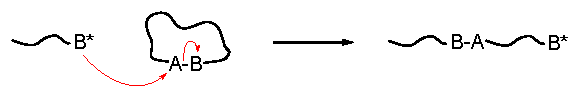
\includegraphics[width=0.7\textwidth]{\figpath/Model1_ROP_general}}
	
	Here, B* denotes the active functional group on the end of the growing polymer chain which is able to attack the A-B bond in the cyclic monomer.
	
	%A specific example of a ring-opening polymerization that you have seen in an earlier activity is anionic polymerization of ethylene oxide, shown below:
	
	%SCHEME
	
\end{model}


\begin{ctqs}

	\question Is the mechanism shown above better described as a chain-growth polymerization or a step-growth polymerization?  Explain your group's reasoning in 1-2 complete sentences.
			
				\begin{solution}[1in]
					This is a \emph{chain-growth} polymerization, because monomers have to add to the end of an active chain (they cannot react directly with each other), and the active site transfers to the end of the monomer that was just added.
				\end{solution}
	
	\question Consider the changes in entropy that occur during this reaction.
	
		\begin{enumerate}
			
			\item Does the \textit{translational} freedom of the monomer increase or decrease during this propagation step?  %Briefly explain your group's reasoning.
			
				\begin{solution}[0.3in]
					The translational freedom of the monomer \textit{decreases} because it is now restricted to moving with the polymer chain.
				\end{solution}
			
			\item Does the \textit{conformational} freedom of the monomer increase or decrease during this propagation step?  %Briefly explain your group's reasoning.
			
				\begin{solution}[0.3in]
					The conformational freedom of the monomer \textit{increases} because it is more flexible once it is no longer constrained to have its two ends connected in a ring.
				\end{solution}
			
			\item Based on your answers to the previous parts of this question, do you expect the overall entropy of the system to increase or decrease during this propagation step?  Briefly explain your group's reasoning.
			
				\emph{Hint: if your answers to parts (a) and (b) were different, which one do you think will be the bigger contribution?}
			
				\begin{solution}[1.25in]
					The overall entropy of the system will \emph{decrease} - the decrease in translational entropy of the monomer is typically much larger than the increase in its conformational entropy.
					
					Note that there are some exceptions to this rule - for very large cyclic molecules (typically 14 or more backbone bonds), the gain in conformational entropy can win out over the translational entropy loss, especially for polymerizations conducted at high monomer concentrations.  This is the basis for entropy-driven ring-opening metathesis polymerization (ED-ROMP).
				\end{solution}
			
		\end{enumerate}

	\question Next, consider the changes in bonding that occur during this propagation reaction.
	
		\begin{enumerate}
		
			\item Is there any \emph{net change} in the number of A-B bonds present in the reaction mixture during this propagation step?
			
				\begin{solution}[0.3in]
					no
				\end{solution}
	
			\item Is there any \emph{net change} in the number of B* reactive sites present in the reaction mixture during this propagation step?
			
				\begin{solution}[0.3in]
					no
				\end{solution}
	
			\item Based on your answers to the previous questions, do you expect changes in the chemical bonding to contribute significantly to the enthalpy of this reaction? Briefly explain your group's reasoning.
			
				\begin{solution}[1.25in]
					No, if there is no net change in the type or number of bonds, then the enthalpy change should be minimal.
				\end{solution}
						
		\end{enumerate}
		
	\question Finally, consider the changes in the \emph{bond angles} that occur during this propagation reaction.
	
		\begin{enumerate}
		
			\item The structures of cyclopropane and cyclobutane are shown below:
			
				\centerline{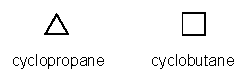
\includegraphics[width=0.4\textwidth]{\figpath/Model1_cyclicmolecules}}
				
				How do the bond angles in these molecules compare to the bond angles you would expect in a linear alkane?
			
				\begin{solution}[1in]
					The bond angles are much smaller (about 60 and 90$^\circ$) than expected in a linear alkane (typically around 109$^\circ$).
				\end{solution}
				
			\item Based on your answer to the previous question, do you expect ``opening up'' a cyclic molecule to form a linear molecule to be enthalpically favorable or enthalpically unfavorable?  Briefly explain your group's reasoning.
			
				\begin{solution}[1in]
					Decreasing bond angles from their preferred configuration typically increases their energy, so opening up a cyclic molecule to form a linear molecule and allowing the bonds to relax back to their energy minimum should be enthalpically favorable.
				\end{solution}
			
		\end{enumerate}
		
	\question Based on your answers to CTQs 1-3, what do you expect is the primary driving force for propagation in a ring-opening polymerization?
			
				\begin{solution}[0.75in]
					Ring-opening polymerization is driven by the enthalpically-favorable \emph{relief of ring strain}.
				\end{solution}

\end{ctqs}

\begin{infobox}

	The \emph{ring strain} of a cyclic molecule can be quantified by comparing the heat of combustion for the cyclic molecule to that expected for a linear alkane of the same length.
	
	The ring strains for several small cyclic alkanes are tabulated below:
	% numbers from: https://chem.libretexts.org/Courses/Siena_Heights_University/SHU_Organic_Chemistry_I/3%3A_Chapter_3_Conformations_and_Cycloalkanes/3.04%3A_Stability_of_Cycloalkanes_-_Ring_Strain
	\begin{center}
	\begin{tabular}{lcc}
		\hline		
		Molecule & \ce{CH2} units & Ring Strain (kcal/mol)\\\hline
		Cyclopropane & 3 & 27.6\\
		Cyclobutane & 4 & 26.4\\
		Cyclopentane & 5 & 6.5\\
		Cyclohexane & 6 & 0.0\\
		Cycloheptane & 7 & 6.3\\
		%Cyclooctane & 8 & 9.6%\\\hline
	\end{tabular}
	\end{center}

\end{infobox}

\begin{ctqs}

	\question Based on these numbers, are there any ring sizes for which ring-opening polymerization should \emph{not} be favorable?  Explain your group's reasoning in 2-3 complete sentences. \label{\labelbase:ctq:ringsizes}
			
				\begin{solution}[2in]
					Ring-opening polymerization should not be favorable for 6-membered rings, because they have negligible ring strain.  Additionally, ring-opening polymerization should be less favorable for five- and seven-membered rings than for 3- and 4-membered rings because they have relatively low ring strain.
					
					Note: this rule strictly only holds for rings composed of only sp\textsuperscript{3} centers - 6-membered rings containing sp\textsuperscript{2} centers (such as lactide) can also have enough ring strain to be polymerizable via ring-opening polymerizations.
				\end{solution}

\end{ctqs}

\clearpage
\begin{model}[Ring-Opening Metathesis]
	\label{\labelbase:mdl:ROMP}

	One type of reaction that is frequently used in ring-opening polymerizations is olefin metathesis.
	In an olefin metathesis reaction, two double bonds ``swap partners'', as shown below:
	
	\centerline{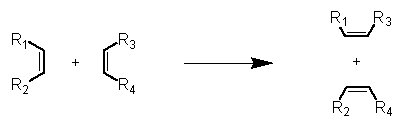
\includegraphics[width=0.6\textwidth]{\figpath/Model2_metathesis_general}}
	
	In polymer chemistry, this process is usually catalyzed by a ruthenium-based catalyst called a Grubbs catalyst.
	
\end{model}

\begin{ctqs}
	
	\question Predict the product of the following metathesis reaction: \label{\labelbase:ctq:metathesis1}
	
		\begin{solution}[1in]\studentdisplay{
			\centerline{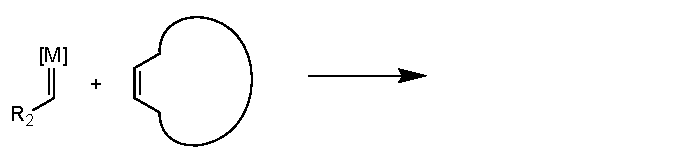
\includegraphics[width=0.75\textwidth]{\figpath/Model2_ROMP_general}}
		}\instructordisplay{
			\centerline{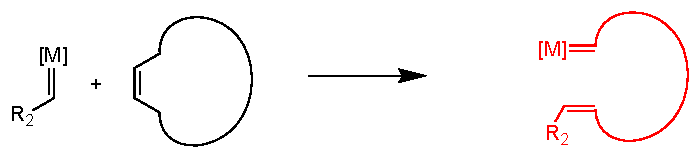
\includegraphics[width=0.75\textwidth]{\figpath/Model2_ROMP_general_answer}}
		}\end{solution}
		
		\emph{Note: here, [M] indicates the location of the metal center of the catalyst.}
		
		\emph{If you are stuck on this question, try replacing R\textsubscript{1} in Model \ref{\labelbase:mdl:ROMP} with [M] and draw a curve connecting R\textsubscript{3} and R\textsubscript{4}!}
		
	\question Compare the reaction you drew in the previous question to the generic ring-opening polymerization reaction in Model \ref{\labelbase:mdl:ROP}, and answer the following:
	
		\begin{enumerate}
			\item In ring-opening metathesis, what species plays the role of the active chain end, B\textsuperscript{*}?
			
				\begin{solution}[0.5in]
					The transition metal alkylidene, =[M]
				\end{solution}
				
			\item In ring-opening metathesis, what type of chemical bond plays the role of the A-B bond?
			
				\begin{solution}[0.5in]
					The C=C double bond
				\end{solution}
				
		\end{enumerate}
		
	\question Based on your answers to the previous question, what type of characteristic bond should appear in the backbone of polymers made using this method?
			
				\begin{solution}[0.5in]
					A C=C double bond
				\end{solution}
	
	\question Propose the structure of the monomer that must have been used to form the following polymer:
	
	\centerline{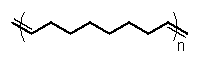
\includegraphics[width=0.25\textwidth]{\figpath/Model2_polycyclooctene}}
			
				\begin{solution}[1.25in]\instructordisplay{
					\centerline{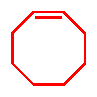
\includegraphics[width=0.15\textwidth]{\figpath/Model2_cyclooctene_answer}}
				}\end{solution}
	
	\question Predict the structure of the polymer that would be formed in a ring-opening metathesis polymerization of norbornene, shown from two angles below:
	
	\centerline{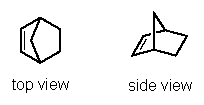
\includegraphics[width=0.3\textwidth]{\figpath/Model2_norbornene}}
			
				\begin{solution}[1.25in]\instructordisplay{
					\centerline{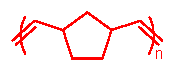
\includegraphics[width=0.25\textwidth]{\figpath/Model2_norbornene_answer}}
					
					If students get stuck, it can help to ask them to envision what would happen if they ``cut the double bond in half''.
				}\end{solution}
	
\end{ctqs}

\vspace{\fill}

\begin{model}[Polylactide]
	\label{\labelbase:mdl:PLA}

	Another common polymer made by ring-opening polymerization is polylactide (PLA).  The mechanism by which a lactide monomer is added to the polymer chain is shown below:
	
	\centerline{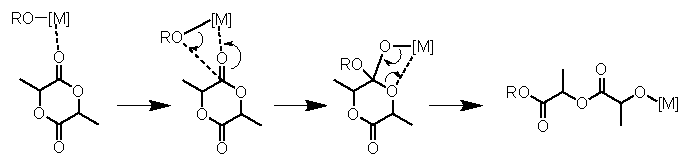
\includegraphics[width=\textwidth]{\figpath/Model3_PLA}}
	
	Here, \ce{[M]} is the metal center of an inorganic catalyst such as tin octoate (\ce{Sn(C8H15O2)2}).
	
\end{model}

\clearpage
\begin{ctqs}
	
	\question Briefly describe what happens to each of the following during the course of this reaction:
	
		\begin{enumerate}
			\item monomer:
			
				\begin{solution}[0.5in]
					The monomer attaches to the metal center and opens up, breaking one ester bond between atoms of the monomer and forming a new ester bond with the RO ligand from the catalyst
				\end{solution}
			
			\item catalyst:
			
				\begin{solution}[0.5in]
					The catalyst coordinates with the monomer and swaps the original RO ligand for a new one originating from the monomer
				\end{solution}
				
		\end{enumerate}
		
	\question Based on the mechanism shown in Model \ref{\labelbase:mdl:PLA}, why do you think this is referred to as a ``coordination-insertion'' polymerization?
			
				\begin{solution}[1in]
					The catalyst coordinates with the monomer, and then the monomer ``inserts'' itself into the bond between the catalyst and its original ligand
				\end{solution}
	
	\question The mechanism shown in Model \ref{\labelbase:mdl:PLA} is a chain-growth polymerization.  However, the resulting polymer could also be prepared \emph{via} a step-growth polymerization as well.
	
		\begin{enumerate}
			\item Propose the structure of the monomer (or monomers) that would be needed to prepare polylactide via a step-growth polymerization.
			
				\begin{solution}[1in]\instructordisplay{
					\centerline{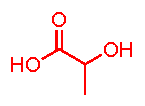
\includegraphics[width=0.15\textwidth]{\figpath/Model3_lactic-acid}}
				}\end{solution}
			
			\item Based on what you remember about the molecular weight distributions of polymers produced by step-growth polymerization, why do you think that most commercial suppliers of PLA prepare it by the chain-growth mechanism shown in Model \ref{\labelbase:mdl:PLA} instead?  Explain your group's reasoning in 2-3 complete sentences.
			
				\begin{solution}[1.5in]
					Recall that step-growth polymerizations produce a lot of low-molecular-weight products, and that esterification reactions can be difficult to drive to high conversion.  The chain-growth mechanism is preferable for its ability to easily access high molecular-weight polymers without extreme reaction conditions.
				\end{solution}
		\end{enumerate}
	
\end{ctqs}




\begin{exercises}

	\exercise In CTQ \ref{\labelbase:ctq:ringsizes}, you (hopefully!) concluded that ring-opening polymerization of 6-membered rings is not favorable.  However, in the polymerization shown in Model \ref{\labelbase:mdl:PLA}, the monomer used (lactide) has 6 atoms in the ring.  Why is it favorable for this monomer to undergo ring-opening polymerization even though it is a 6-membered ring?
	
		\emph{Hint: is the 6-membered ring in lactide equivalent to the 6-membered ring in cyclohexane?  If not, what is different?}
	
		\begin{solution}\instructordisplay{
			Cyclohexane is a cyclic alkane, with sp\textsuperscript{3} hybridized carbons in all 6 positions.  Lactide, however, is a cyclic ester, containing two sp\textsuperscript{2} hybridized carbons at the base of the C=O bonds.  Because these sites prefer to have a bond angle closer to 120$^\circ$ rather than 109$^\circ$, they do not naturally fall into the 6-membered ring geometry and the molecule does indeed end up with not-insignificant angle strain.
			
			Additionally, upon ring opening, the esters are able to switch their conformations from the (E) conformation to the (Z) conformation, which is typically energetically favorable.
		}\end{solution}
	
\end{exercises}


%\begin{problems}
%
%	\problem First exercise
%	\problem Second exercise
%	
%\end{problems}


	
\end{activity}